\documentclass[conference]{IEEEtran}
\IEEEoverridecommandlockouts

\usepackage{cite}
\usepackage{amsmath,amssymb}
\usepackage{graphicx}
\usepackage{booktabs}
\usepackage{array}
\usepackage{tabularx}
\usepackage{xcolor}
\usepackage{url}
\usepackage{tikz}
\usetikzlibrary{arrows.meta,positioning}

% ------------------------------------------------------------------
% PROJECT DETAILS
% ------------------------------------------------------------------
\newcommand{\institute}{Rishihood University}
\DeclareRobustCommand{\repolink}{\url{https://github.com/aman01k/Turtle-Graphics-Compiler}}
% ------------------------------------------------------------------

\graphicspath{{figures/}}
\newcommand{\kw}[1]{\texttt{#1}}

\begin{document}

\title{Turtle Graphics Compiler: A Six-Phase Compiler with Phase-by-Phase Interactive Visualization}

\author{
\IEEEauthorblockN{Aman}
\IEEEauthorblockA{Enrollment No. 230065\\
\institute}
\and
\IEEEauthorblockN{Asmit}
\IEEEauthorblockA{Enrollment No. 230063\\
\institute}
\and
\IEEEauthorblockN{Shashwat}
\IEEEauthorblockA{Enrollment No. 230127\\
\institute}
\thanks{Compiler Design course project. Source code: \protect\repolink}
}

\maketitle

\begin{abstract}
This report presents the Turtle Graphics Compiler, a complete compiler for a small domain-specific language that describes line drawings. A program is a sequence of commands such as \kw{PEN BLUE}, \kw{MOVE 100} and \kw{TURN 90}, with named constants, arithmetic expressions and nested \kw{REPEAT} loops. The compiler implements all six classical phases: lexical analysis, syntax analysis, semantic analysis, intermediate code generation, optimization and code generation. The target language is Scalable Vector Graphics (SVG), which a web browser displays directly. The compiler is delivered as a web application that needs no installation. As the user types, the application shows the output of every phase: the token list, the abstract syntax tree, the symbol table, the intermediate code, the optimized code, the generated SVG and the final drawing. Errors are detected in three phases and reported with line and column numbers, and the lexer and parser recover from errors so that several are reported in one run. A suite of 47 automated tests covers correct programs and error cases for every phase. On a deliberately wasteful test program the optimizer reduces the intermediate code from 18 instructions to 7.
\end{abstract}

\begin{IEEEkeywords}
compiler design, domain-specific language, turtle graphics, recursive descent parsing, symbol table, intermediate representation, peephole optimization, SVG
\end{IEEEkeywords}

\section{Introduction}
A compiler translates a program written in a source language into an equivalent program in a target language. The translation is organised as a pipeline of phases, each of which takes the output of the previous one \cite{aho}. These phases are usually taught with general-purpose languages, where the size of the language hides the structure of the pipeline.

This project uses a much smaller language. Turtle graphics, introduced with the Logo language \cite{papert}, describes a drawing as the path of a ``turtle'' that carries a pen. The turtle moves forward, turns and lifts or lowers its pen. The language is small enough to be understood completely, yet it needs every phase of a real compiler: it has keywords and numbers to scan, nested blocks and expressions to parse, declarations and value ranges to check, loops to lower into simpler code, redundant instructions to optimize away and a target format to generate.

The project has two goals:
\begin{itemize}
\item to build a correct compiler from the turtle language to SVG, with error handling in the lexical, syntax and semantic phases;
\item to make the intermediate result of every phase visible, so that a user can follow one program through the whole pipeline.
\end{itemize}

The project follows the AI Product Engineering Track of the course. A generative AI assistant was used to produce the implementation under the direction of the team, who chose the language, reviewed the code of each module and tested the result.

The rest of this report is organised as follows. Section~\ref{sec:lang} defines the language. Section~\ref{sec:method} describes the design of each phase. Section~\ref{sec:impl} covers the implementation and the user interface. Section~\ref{sec:errors} lists the errors handled. Section~\ref{sec:results} gives the results. Section~\ref{sec:contrib} states the contribution of each member, and Sections~\ref{sec:future} and~\ref{sec:concl} give the future scope and the conclusion.

\section{The Source Language}\label{sec:lang}

\subsection{Statements}
Table~\ref{tab:stmts} lists the eight statements of the language. Every value can be an arithmetic expression that uses \kw{+}, \kw{-}, \kw{*}, \kw{/}, parentheses and unary minus, for example \kw{MOVE size * 2 + 10;}. A comment starts with \kw{\#} and runs to the end of the line. Keywords and colour names are case-insensitive, and variable names are case-sensitive.

\begin{table}[htbp]
\caption{Statements of the Turtle Language}
\label{tab:stmts}
\centering
\footnotesize
\begin{tabularx}{\columnwidth}{@{}l>{\raggedright\arraybackslash}X>{\raggedright\arraybackslash}p{2.3cm}@{}}
\toprule
Statement & Meaning & Semantic rule\\
\midrule
\kw{PEN BLUE;} & Set the pen colour & One of 12 colours\\
\kw{MOVE 100;} & Go forward; negative goes backward & $-1000$ to $1000$\\
\kw{TURN 90;} & Turn right; negative turns left & $-360$ to $360$\\
\kw{WIDTH 3;} & Set the line thickness & $1$ to $20$\\
\kw{PENUP;} & Move without drawing & --\\
\kw{PENDOWN;} & Draw while moving & --\\
\kw{LET s = 50;} & Declare a named constant & Once per scope, before use\\
\kw{REPEAT 4 \{...\}} & Run a block several times & Whole number, $1$ to $1000$\\
\bottomrule
\end{tabularx}
\end{table}

The turtle starts at the origin, facing up, with a black pen of width 2 that is down. The following program draws a blue square:

\begin{verbatim}
PEN BLUE;
REPEAT 4 {
  MOVE 100;
  TURN 90;
}
\end{verbatim}

\subsection{Grammar}
The context-free grammar of the language is given below. It is LL(1): one token of lookahead is enough to choose a production.

{\footnotesize
\begin{verbatim}
program   -> statement* EOF
statement -> PEN IDENT ';'
           | MOVE expr ';'
           | TURN expr ';'
           | WIDTH expr ';'
           | PENUP ';'
           | PENDOWN ';'
           | LET IDENT '=' expr ';'
           | REPEAT expr '{' statement* '}'
expr      -> term (('+' | '-') term)*
term      -> factor (('*' | '/') factor)*
factor    -> NUMBER | IDENT
           | '(' expr ')' | '-' factor
\end{verbatim}
}

Operator precedence is encoded in the grammar. Because \textit{term} is below \textit{expr}, multiplication and division bind tighter than addition and subtraction. The repetition in each rule makes the binary operators left-associative.

\section{Methodology}\label{sec:method}

\subsection{Architecture}
Fig.~\ref{fig:pipeline} shows the pipeline. Each phase is a separate module with one input and one output, and a driver module runs them in order. If a phase reports an error, the driver stops, because later phases cannot work on an invalid program. The results of the phases that did run are still shown to the user.

\begin{figure}[htbp]
\centering
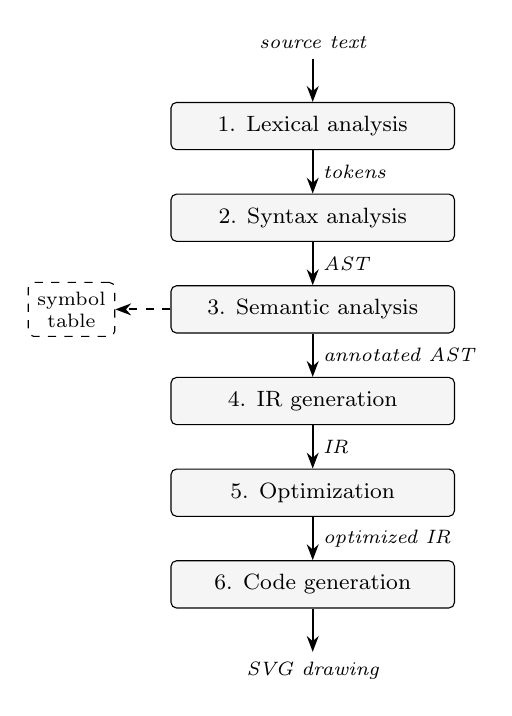
\begin{tikzpicture}[
  node distance=5.5mm,
  phase/.style={draw, rounded corners=2pt, minimum width=3.6cm, minimum height=6mm, font=\footnotesize, fill=black!4},
  data/.style={font=\scriptsize\itshape},
  arr/.style={-{Stealth[length=2mm]}, thick}]
\node[data] (src) {source text};
\node[phase, below=of src] (lex) {1. Lexical analysis};
\node[phase, below=of lex] (syn) {2. Syntax analysis};
\node[phase, below=of syn] (sem) {3. Semantic analysis};
\node[phase, below=of sem] (ir) {4. IR generation};
\node[phase, below=of ir] (opt) {5. Optimization};
\node[phase, below=of opt] (gen) {6. Code generation};
\node[data, below=of gen] (out) {SVG drawing};
\draw[arr] (src) -- (lex);
\draw[arr] (lex) -- node[right, data] {tokens} (syn);
\draw[arr] (syn) -- node[right, data] {AST} (sem);
\draw[arr] (sem) -- node[right, data] {annotated AST} (ir);
\draw[arr] (ir) -- node[right, data] {IR} (opt);
\draw[arr] (opt) -- node[right, data] {optimized IR} (gen);
\draw[arr] (gen) -- (out);
\node[draw, dashed, rounded corners=2pt, font=\scriptsize, align=center, left=7mm of sem] (st) {symbol\\table};
\draw[arr, dashed] (sem) -- (st);
\end{tikzpicture}
\caption{The six phases of the compiler and the data passed between them.}
\label{fig:pipeline}
\end{figure}

\subsection{Phase 1: Lexical Analysis}
The lexer is a hand-written scanner. It reads the source one character at a time and groups characters into tokens of 14 types: \kw{KEYWORD}, \kw{IDENT}, \kw{NUMBER}, \kw{SEMI}, \kw{LBRACE}, \kw{RBRACE}, \kw{LPAREN}, \kw{RPAREN}, \kw{ASSIGN}, \kw{PLUS}, \kw{MINUS}, \kw{STAR}, \kw{SLASH} and \kw{EOF}. Whitespace and comments are discarded. Each token stores its type, its lexeme and the line and column where it starts, which later phases use to report errors.

A word is looked up in the list of eight reserved words. If it is found, the token is a \kw{KEYWORD}, and otherwise it is an \kw{IDENT}. Colour names are scanned as identifiers and are validated later, in semantic analysis.

\subsection{Phase 2: Syntax Analysis}
The parser uses recursive descent \cite{aho}, a top-down method in which every grammar rule becomes one function. The function for \textit{statement} looks at the current keyword to decide which statement to parse. The functions for \textit{expr}, \textit{term} and \textit{factor} call one another in the order given by the grammar. The output is an abstract syntax tree (AST) with 13 node types, such as \kw{Program}, \kw{Move}, \kw{Let}, \kw{Repeat}, \kw{BinOp}, \kw{Number} and \kw{Var}. Fig.~\ref{fig:ast} shows the tree for the square program.

\begin{figure}[htbp]
\centering
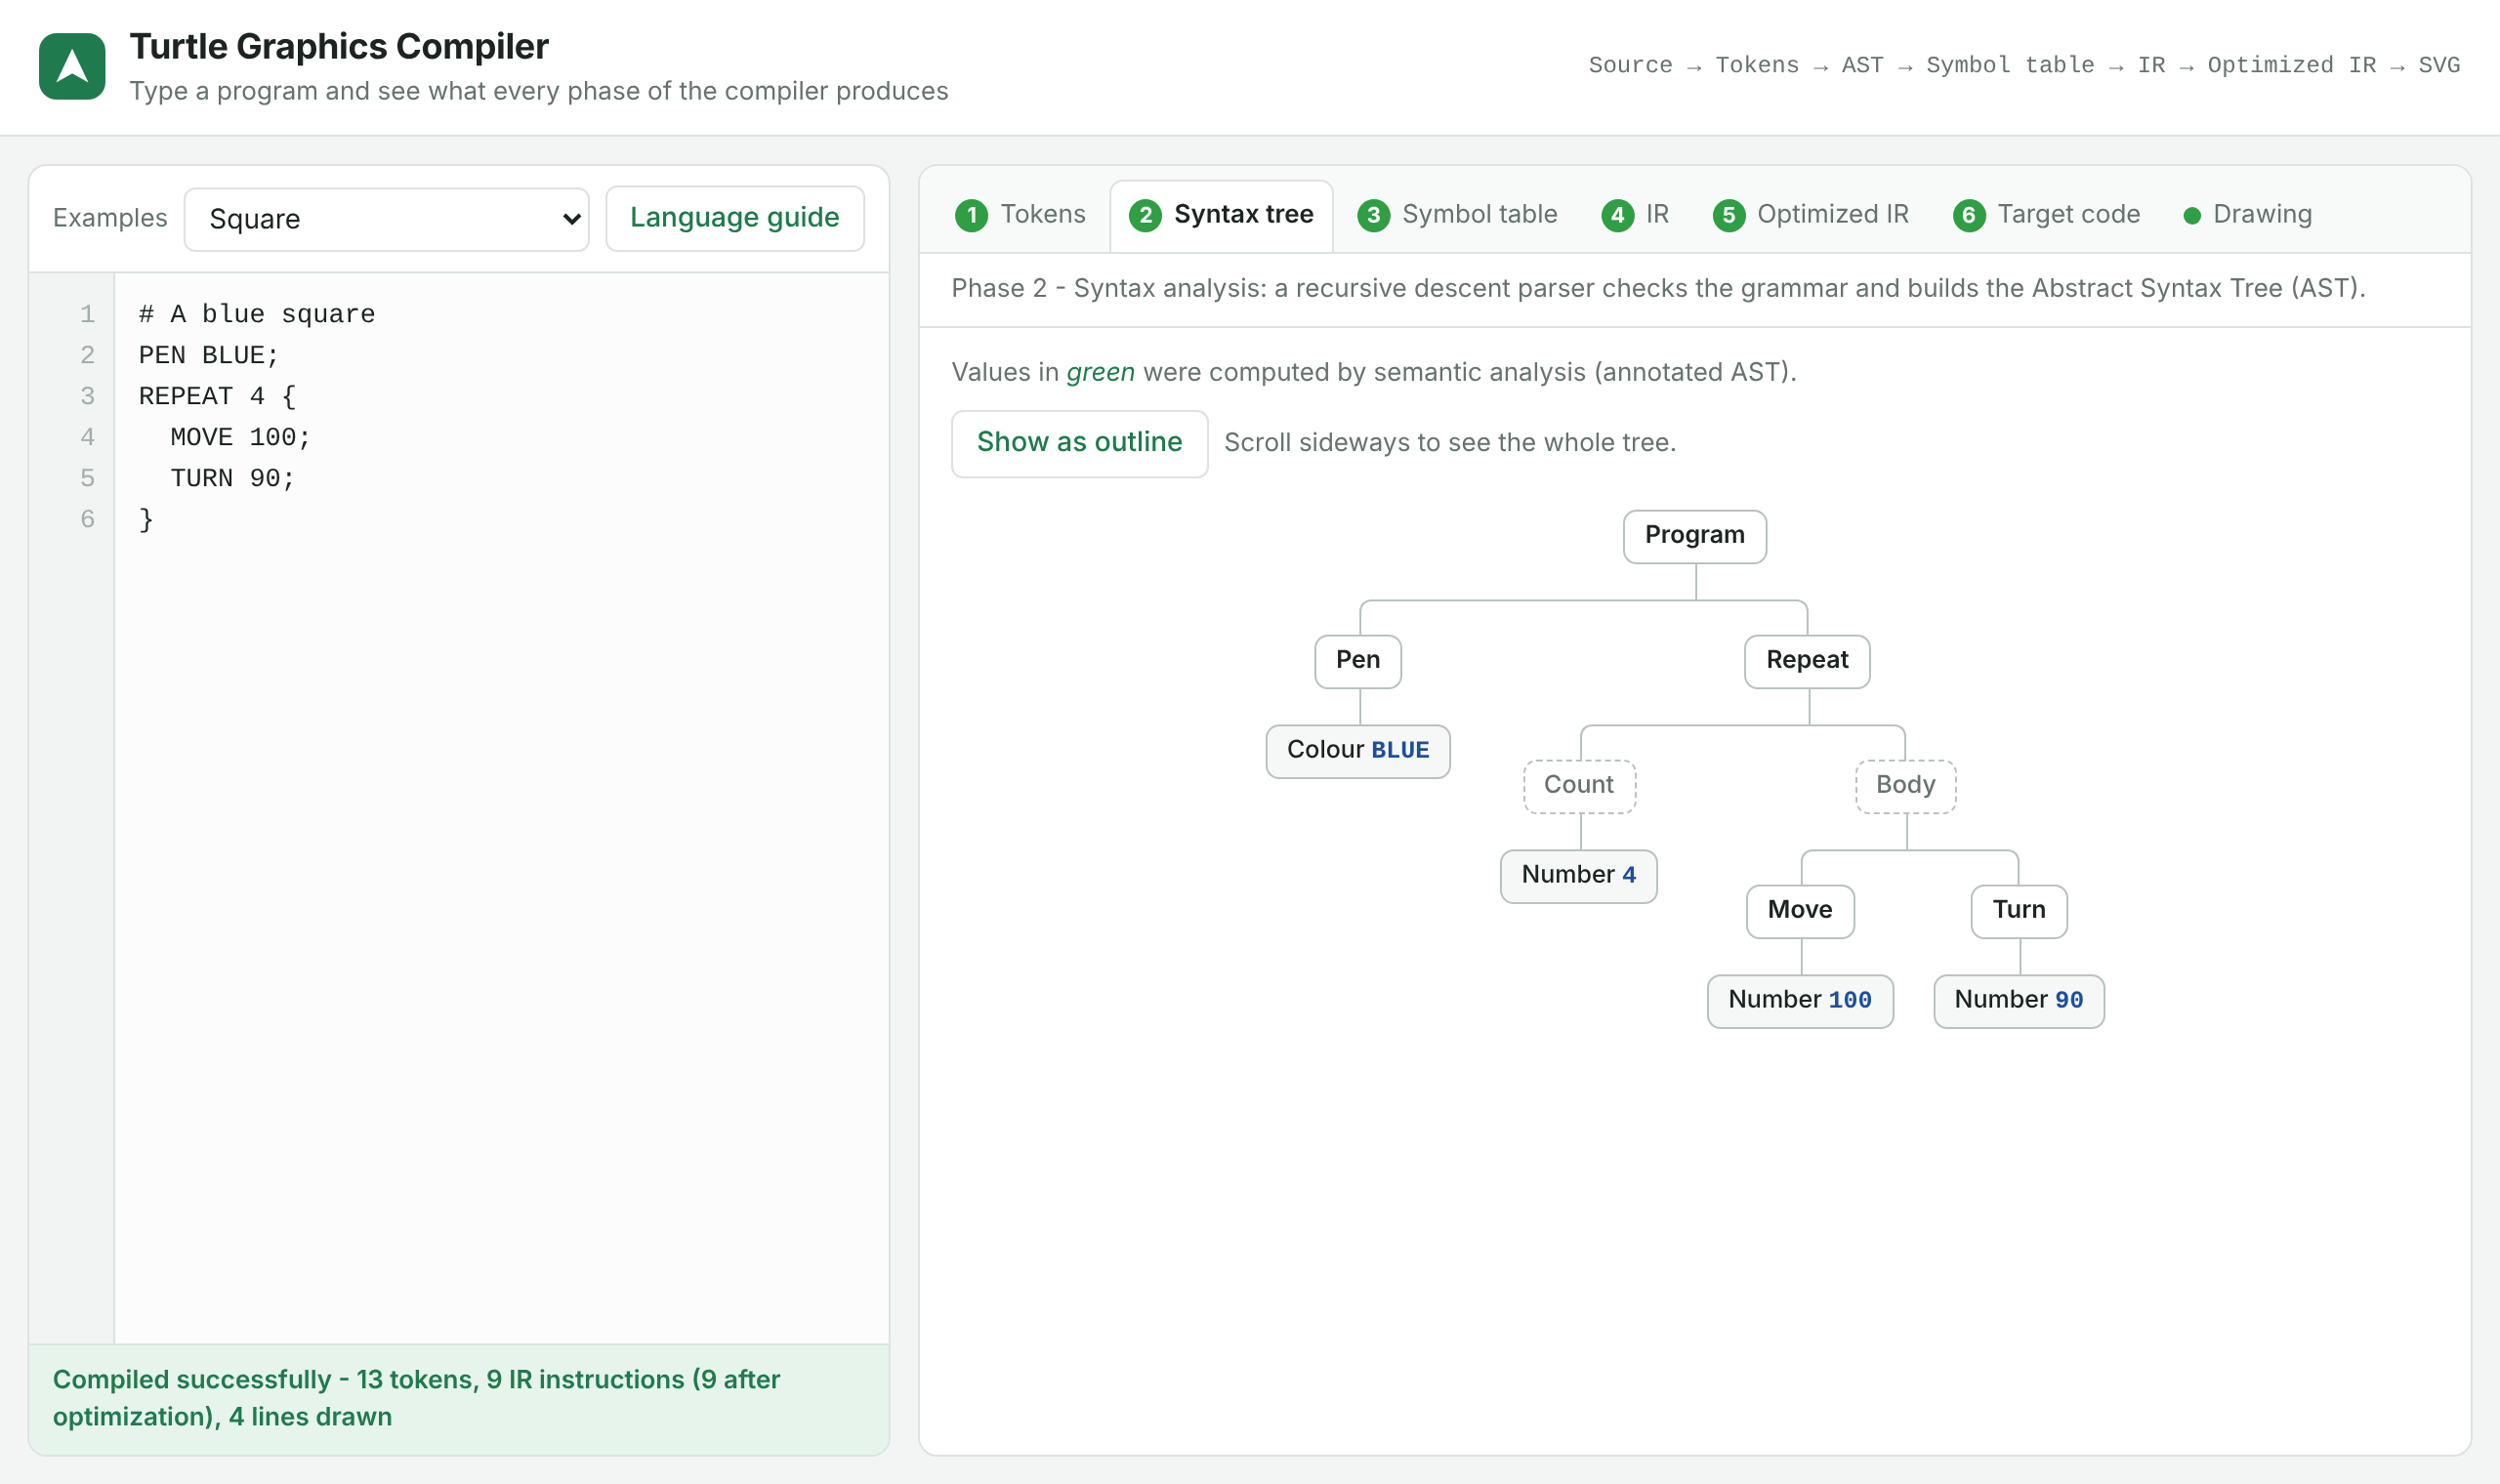
\includegraphics[width=\columnwidth]{fig-ast.png}
\caption{The syntax tree tab, showing the AST of the square program.}
\label{fig:ast}
\end{figure}

\subsection{Phase 3: Semantic Analysis}
The semantic analyser walks the AST and checks the rules that a grammar cannot express. It keeps a stack of scopes. The program body is the global scope, and each \kw{REPEAT} block opens an inner scope. A name is looked up from the innermost scope outwards, so an inner declaration may shadow an outer one, and a variable declared inside a block cannot be used after it.

For each \kw{LET} statement the analyser adds an entry to the symbol table with the name, kind, type, value, scope, nesting level, line of declaration and number of uses. A variable is given its value once and cannot be reassigned. For this reason every expression can be evaluated at compile time. The analyser stores the computed value on each expression node, which gives an annotated AST, and uses these values to check the ranges in Table~\ref{tab:stmts}.

\subsection{Phase 4: Intermediate Code Generation}
The intermediate representation (IR) is a linear list of instructions, similar to a small bytecode. It has six instruction kinds: \kw{PEN}, \kw{MOVE}, \kw{TURN}, \kw{WIDTH}, \kw{PENUP} and \kw{PENDOWN}. The generator removes the two structured features of the source language:
\begin{itemize}
\item \textit{Constant folding}: each expression is replaced by the value computed in Phase~3, so a \kw{LET} statement produces no instruction.
\item \textit{Loop unrolling}: the body of a \kw{REPEAT} loop is emitted once for every iteration.
\end{itemize}
For example, \kw{REPEAT 2 \{ MOVE 10; TURN 90; \}} becomes \kw{MOVE 10}, \kw{TURN 90}, \kw{MOVE 10}, \kw{TURN 90}. The IR therefore has no nesting, no variables and no expressions, which makes the next two phases simple. The semantic phase rejects a program that would unroll to more than 20\,000 instructions.

\subsection{Phase 5: Optimization}
The optimizer applies five peephole passes \cite{cooper}. Each pass looks at neighbouring instructions and replaces them with a shorter equivalent. Table~\ref{tab:passes} lists the passes.

\begin{table}[htbp]
\caption{Optimization Passes}
\label{tab:passes}
\centering
\footnotesize
\begin{tabularx}{\columnwidth}{@{}l>{\raggedright\arraybackslash}X@{}}
\toprule
Pass & Example\\
\midrule
Remove no-ops & \kw{MOVE 0} and \kw{TURN 360} are deleted\\
Merge turns & \kw{TURN 30}, \kw{TURN 60} $\rightarrow$ \kw{TURN 90}\\
Merge moves & \kw{MOVE 50}, \kw{MOVE 50} $\rightarrow$ \kw{MOVE 100}\\
Remove redundant sets & \kw{PEN RED} is deleted when the pen is already red\\
Remove dead sets & \kw{PEN RED}, \kw{PEN BLUE} $\rightarrow$ \kw{PEN BLUE}\\
\bottomrule
\end{tabularx}
\end{table}

One pass can create an opportunity for another. Deleting a \kw{TURN 0}, for example, can leave two moves next to each other. The passes are therefore repeated until a full round changes nothing, that is, until a fixed point is reached.

Each pass must keep the drawing unchanged. With the pen down, \kw{MOVE 50} followed by \kw{MOVE -50} draws a line and returns, so the two cannot be merged into \kw{MOVE 0}. The merge-moves pass tracks the pen state and merges moves in opposite directions only when the pen is up.

\subsection{Phase 6: Code Generation}
The target language is SVG \cite{svg}. The generator simulates the turtle over the optimized IR. It keeps the position $(x, y)$, the heading $\theta$, the pen state, the colour and the width. For a move of distance $d$ the new position is
\begin{equation}
x' = x + d\sin\theta, \qquad y' = y - d\cos\theta,
\end{equation}
where the minus sign is needed because the $y$ axis of SVG points down. If the pen is down, the generator emits one \kw{<line>} element from $(x, y)$ to $(x', y')$ with the current colour and width. The \kw{viewBox} of the image is set to the bounding box of the drawing plus a margin, so every picture is centred and scaled to fit.

\section{Implementation}\label{sec:impl}
The compiler is written in JavaScript without any library or build step, and the interface uses HTML and CSS. It runs entirely in the browser: opening \kw{index.html} is enough to use it. Each phase is in its own file (\kw{lexer.js}, \kw{parser.js}, \kw{semantic.js}, \kw{ir.js}, \kw{optimizer.js}, \kw{codegen.js}), and \kw{compiler.js} is the driver. The project has about 2200 lines of code, including the interface and the tests.

Fig.~\ref{fig:ui} shows the interface. The left side holds the editor, a menu of nine example programs and the list of errors and warnings. The right side has one tab per phase. Each tab carries a status mark that is green if the phase succeeded, red if it failed and grey if it was not reached. The program is recompiled on every change, so the effect of an edit on each phase is seen immediately. The drawing tab can replay the drawing one move at a time.

\begin{figure*}[htbp]
\centering
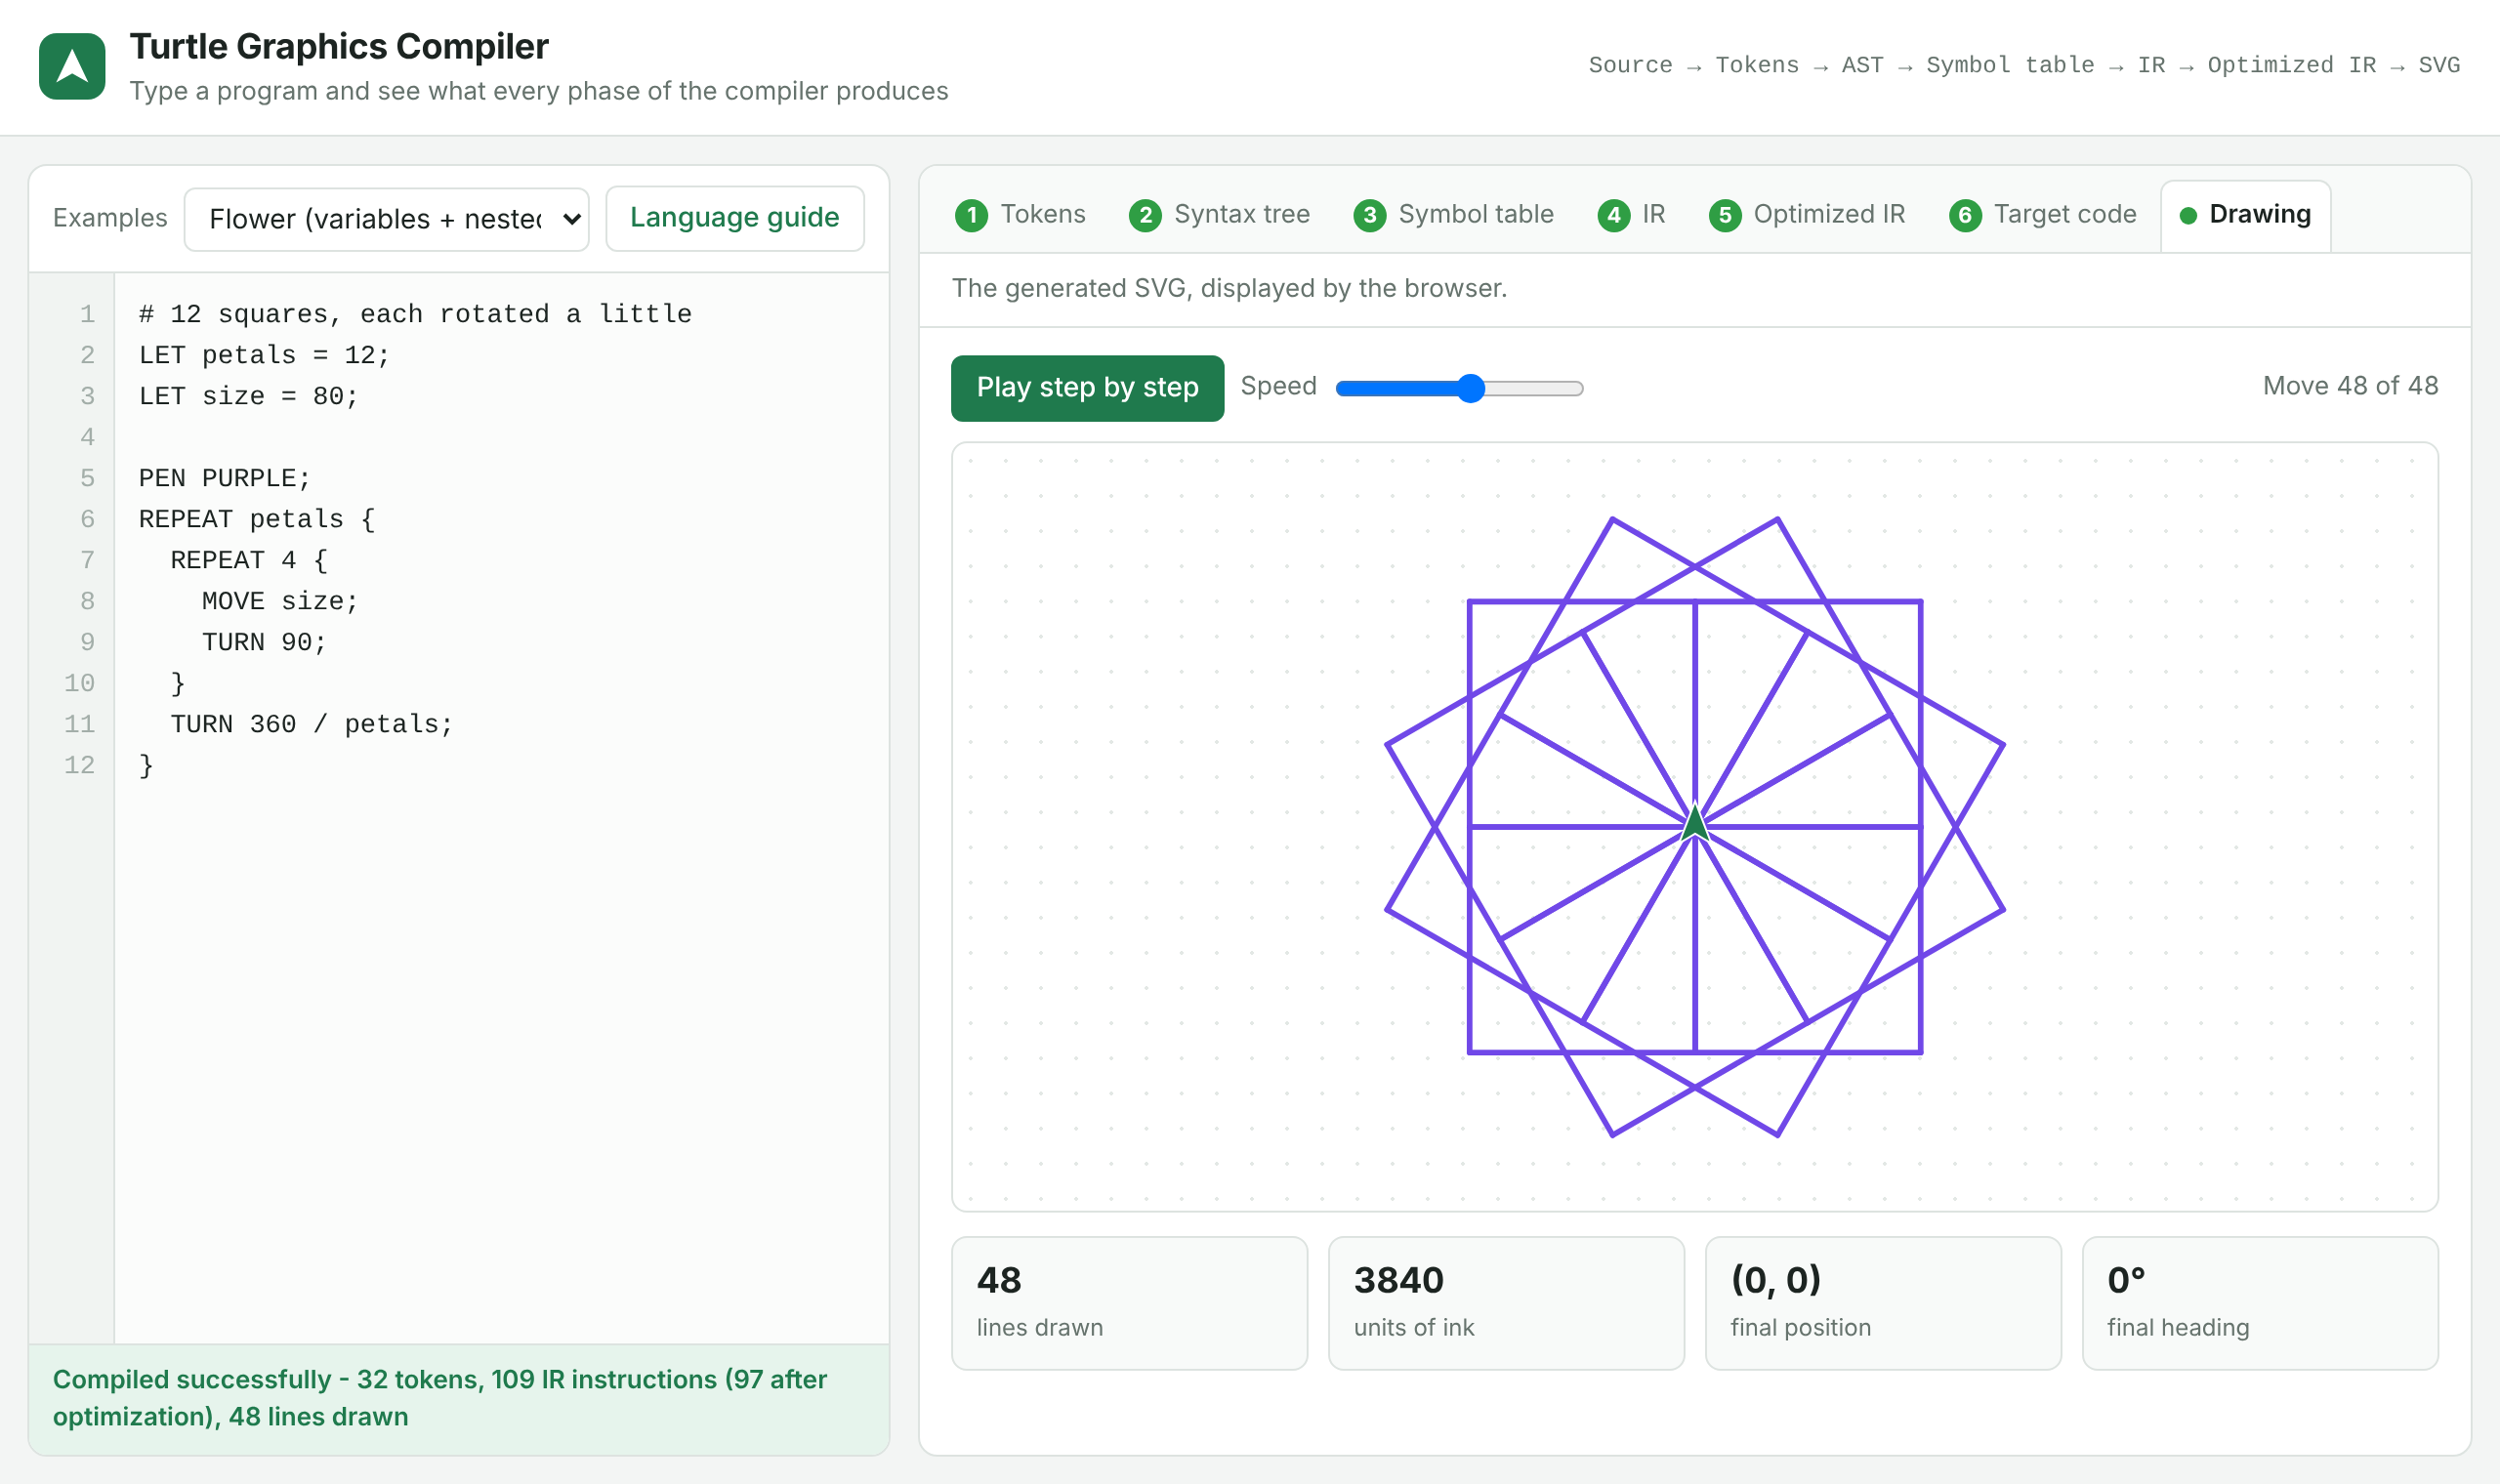
\includegraphics[width=0.86\textwidth]{fig-ui.png}
\caption{The user interface. The editor is on the left. The tabs on the right show the tokens, syntax tree, symbol table, IR, optimized IR, target code and drawing.}
\label{fig:ui}
\end{figure*}

\section{Error Handling}\label{sec:errors}
Errors are detected in three phases. Table~\ref{tab:errors} lists them. Every message gives the phase, the line and the column, and clicking a message moves the cursor to that position.

\begin{table}[htbp]
\caption{Errors Detected in Each Phase}
\label{tab:errors}
\centering
\footnotesize
\begin{tabularx}{\columnwidth}{@{}l>{\raggedright\arraybackslash}X@{}}
\toprule
Phase & Errors\\
\midrule
Lexical & Illegal character; name that starts with a digit\\
Syntax & Missing \kw{;}; missing \kw{\{} or \kw{\}}; stray \kw{\}}; missing value; unknown command; missing \kw{=} in \kw{LET}\\
Semantic & Unknown colour; \kw{MOVE}, \kw{TURN} or \kw{WIDTH} out of range; \kw{REPEAT} count not a positive whole number; undeclared variable; variable used outside its scope; duplicate declaration; division by zero; program too large\\
Warnings & Unused variable; empty \kw{REPEAT} block\\
\bottomrule
\end{tabularx}
\end{table}

The compiler does not stop at the first error within a phase. The lexer skips an invalid character and continues. The parser uses panic-mode recovery \cite{aho}: after an error it skips tokens up to the next semicolon, keyword or closing brace and resumes parsing there. The semantic analyser records an error and continues with the next statement. Fig.~\ref{fig:err} shows seven semantic errors reported in one run.

\begin{figure}[htbp]
\centering
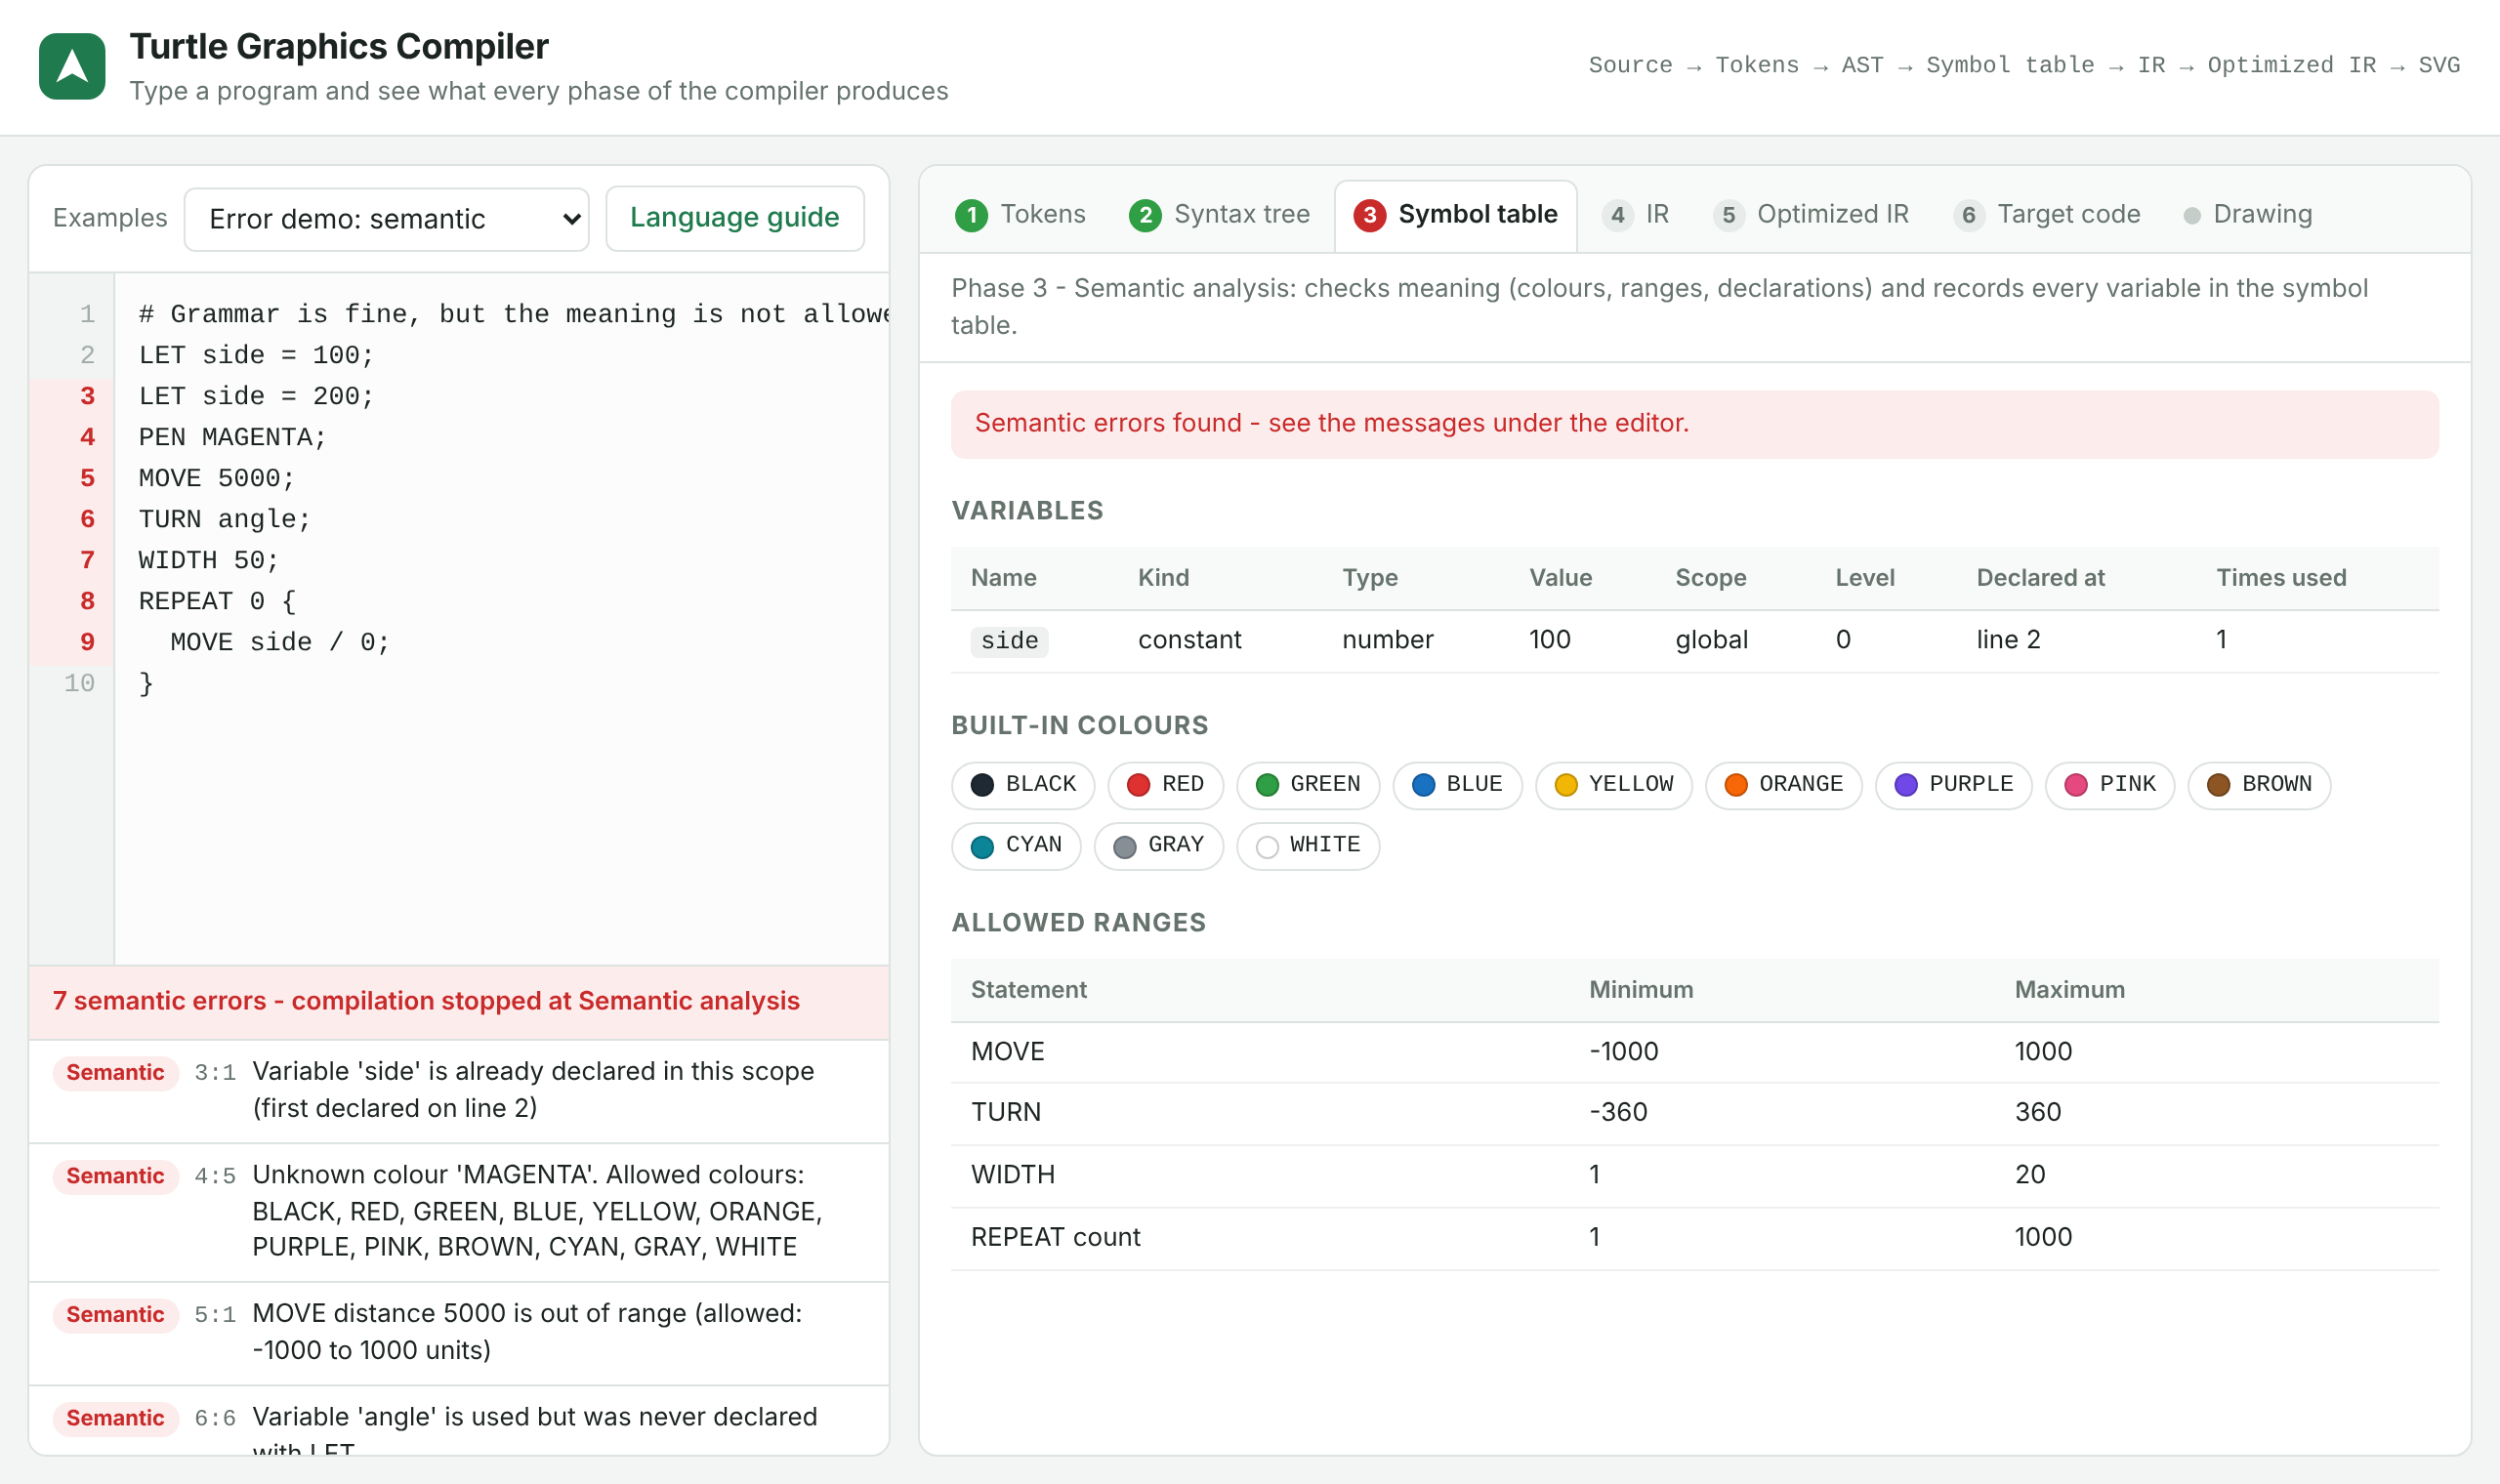
\includegraphics[width=\columnwidth]{fig-err.png}
\caption{Seven semantic errors reported in a single run. The pipeline stops at Phase 3, and the later tabs are marked as not reached.}
\label{fig:err}
\end{figure}

\section{Results}\label{sec:results}

\subsection{Testing}
The test suite has 47 automated tests, which all pass. Table~\ref{tab:tests} gives the number of tests for each phase. The tests check correct output, such as the token types of a program, the value of \kw{2 + 3 * 4} and the end points of the generated lines, and they check that each error in Table~\ref{tab:errors} is reported in the correct phase.

\begin{table}[htbp]
\caption{Automated Tests}
\label{tab:tests}
\centering
\footnotesize
\begin{tabular}{@{}lc@{}}
\toprule
Phase & Tests\\
\midrule
Lexical analysis & 7\\
Syntax analysis & 10\\
Semantic analysis & 14\\
IR generation & 2\\
Optimization & 9\\
Code generation & 5\\
\midrule
Total & 47\\
\bottomrule
\end{tabular}
\end{table}

One test compiles a program with and without optimization and compares the final position and heading of the turtle, the total length drawn and the bounding box. The results are identical, which supports the claim that the optimizer preserves the drawing.

\subsection{Example Programs}
Table~\ref{tab:examples} gives the size of each phase's output for the six valid example programs. The optimizer removes 61\% of the instructions of the program written to exercise it (Fig.~\ref{fig:opt}) and 11\% of the flower program, where it merges the turn that ends each square with the turn that follows it. Four programs are already minimal and are left unchanged.

\begin{table}[htbp]
\caption{Output Sizes for the Example Programs}
\label{tab:examples}
\centering
\footnotesize
\begin{tabular}{@{}lcccc@{}}
\toprule
Program & Tokens & IR & Optimized IR & Lines drawn\\
\midrule
Square & 13 & 9 & 9 & 4\\
Star & 16 & 12 & 12 & 5\\
Flower & 32 & 109 & 97 & 48\\
Dashed triangle & 35 & 102 & 102 & 24\\
House & 46 & 16 & 16 & 7\\
Optimizer demo & 27 & 18 & 7 & 3\\
\bottomrule
\end{tabular}
\end{table}

\begin{figure}[htbp]
\centering
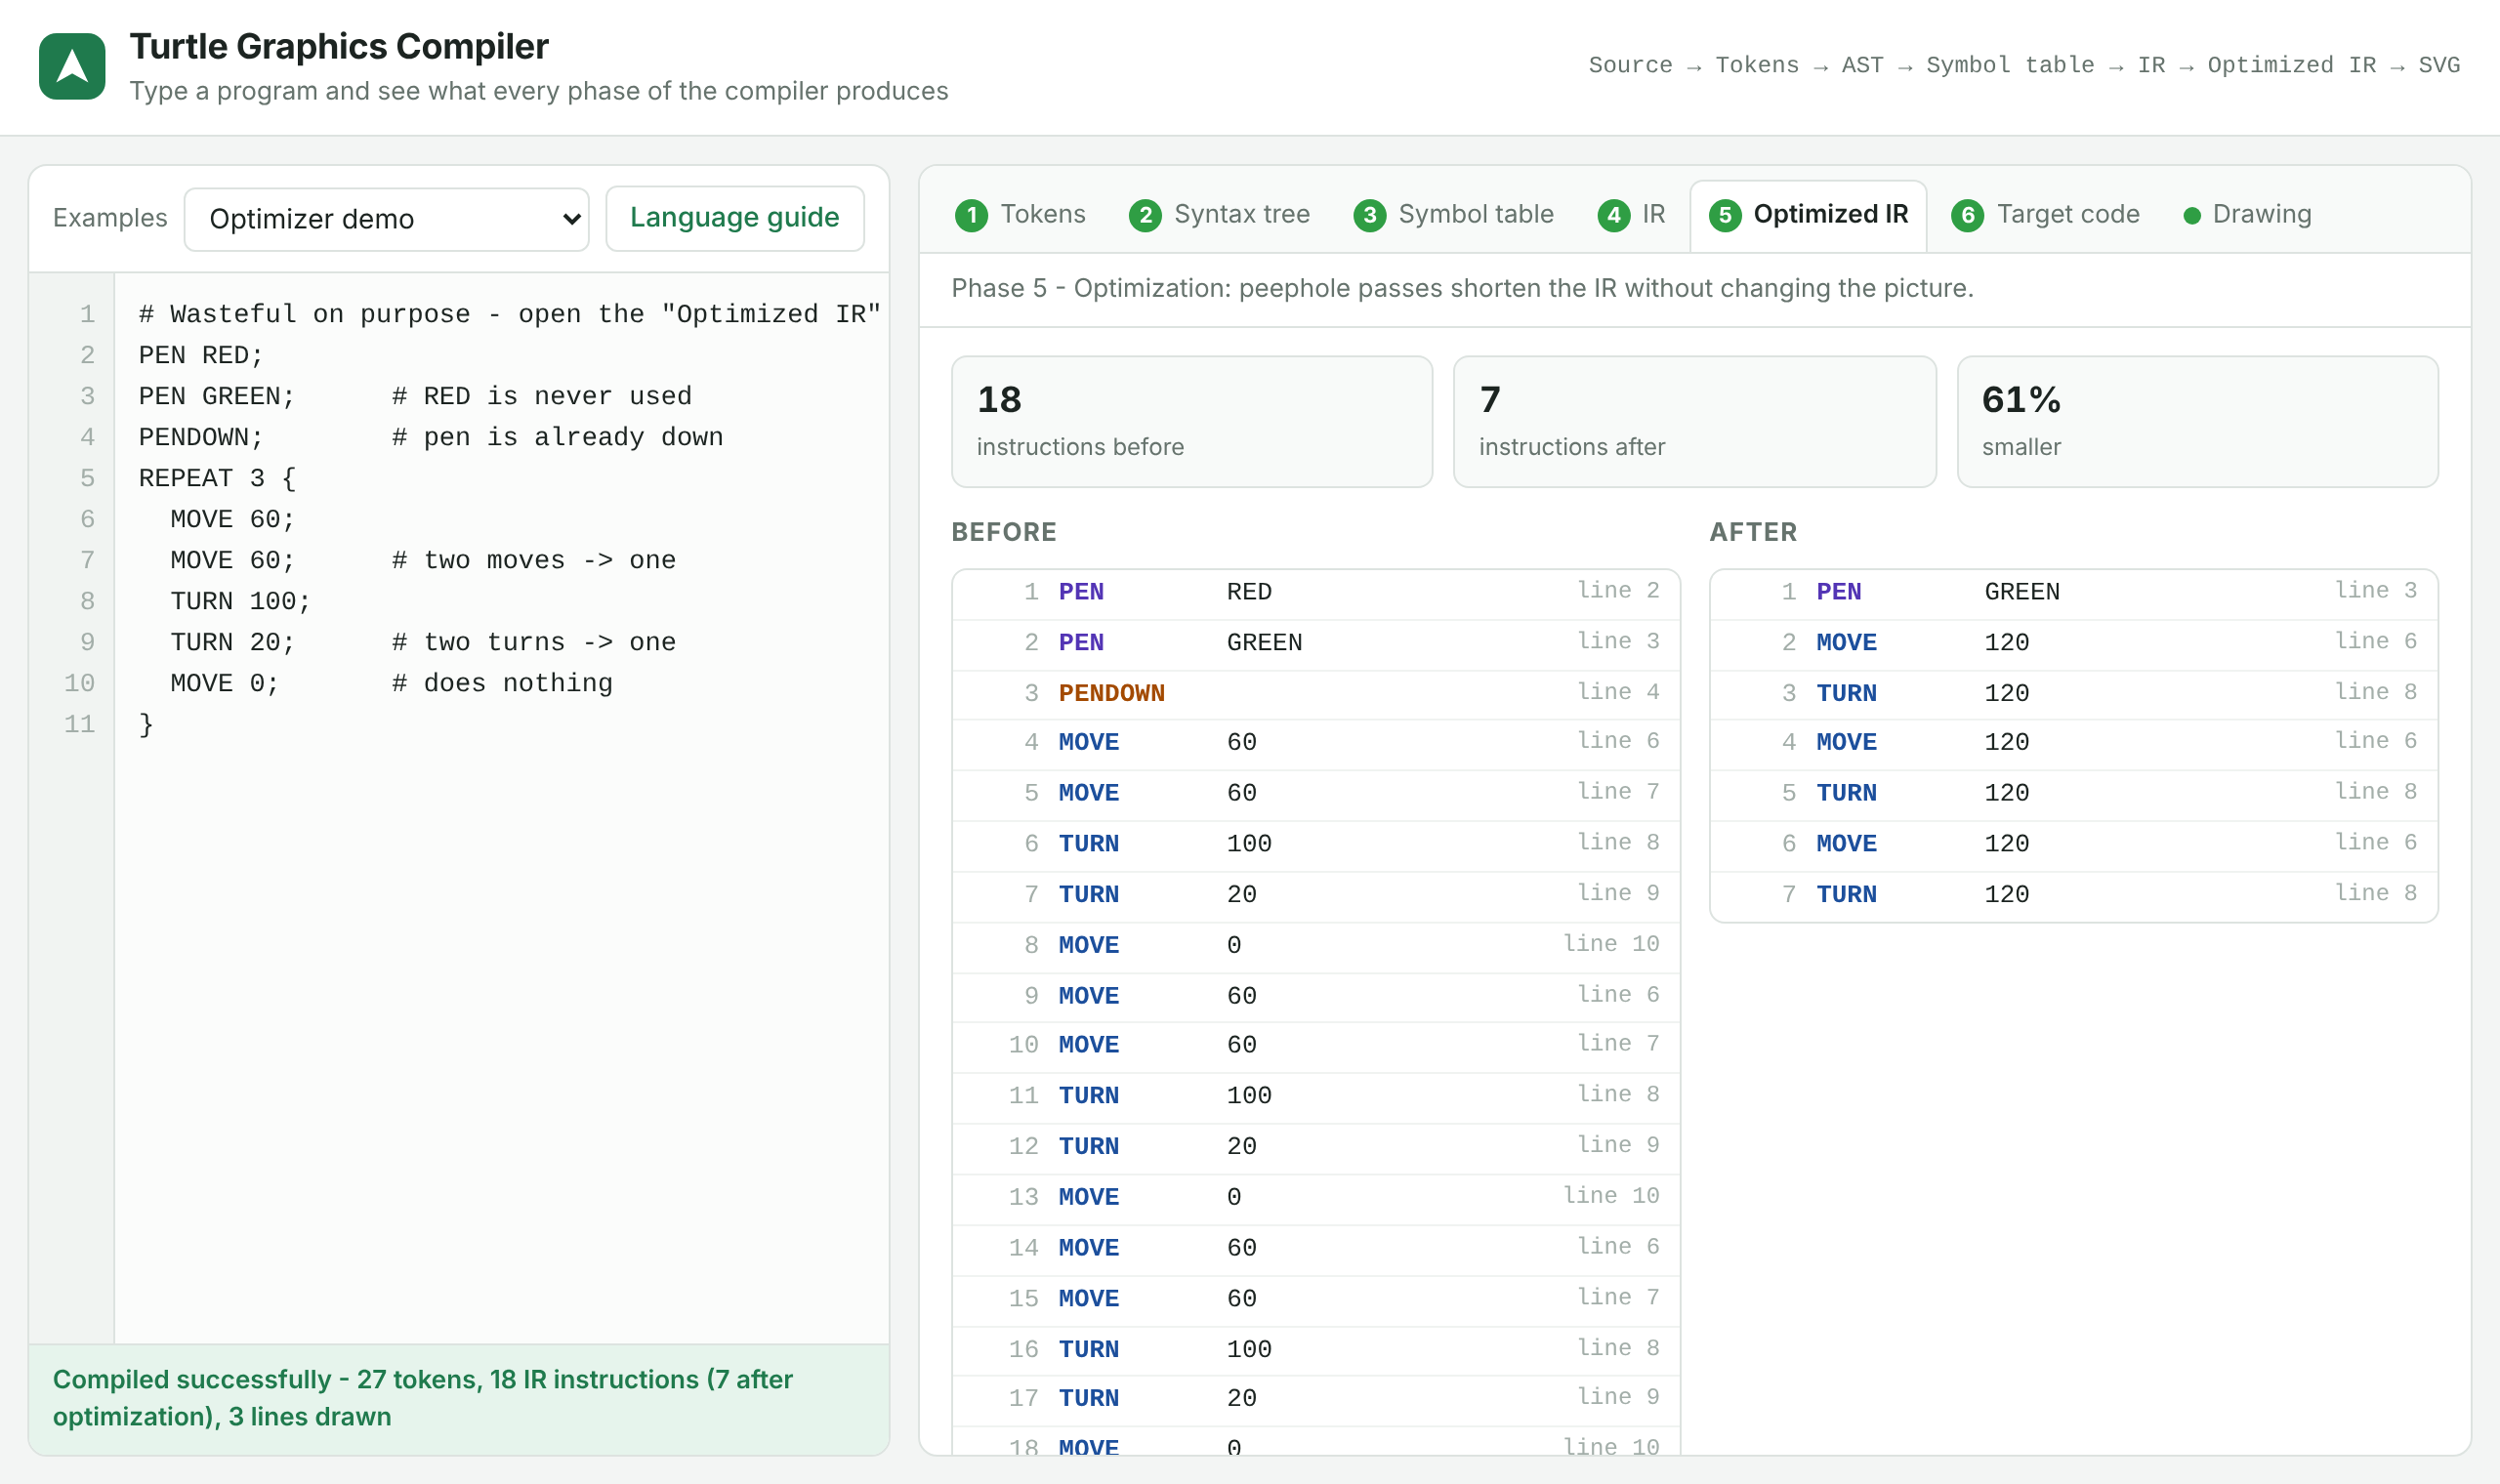
\includegraphics[width=\columnwidth]{fig-opt.png}
\caption{The optimized IR tab for the optimizer demo: 18 instructions are reduced to 7.}
\label{fig:opt}
\end{figure}

The three remaining examples contain deliberate errors. The compiler reports 3 lexical errors, 5 syntax errors and 7 semantic errors for them, each at the correct line and column.

\section{Individual Member Contribution}\label{sec:contrib}
Table~\ref{tab:contrib} gives the modules for which each member was responsible. As stated in Section~I, the code was produced with a generative AI assistant. For the listed modules, each member specified the required behaviour, reviewed the generated code and tested it. The choice of project and the design of the language were made by the team together.

\begin{table}[htbp]
\caption{Contribution of Each Member}
\label{tab:contrib}
\centering
\footnotesize
\begin{tabularx}{\columnwidth}{@{}l>{\raggedright\arraybackslash}X@{}}
\toprule
Member & Modules\\
\midrule
Aman (230065) & Lexical analysis (\kw{lexer.js}); syntax analysis and grammar (\kw{parser.js}); tests for these phases\\
Asmit (230063) & Semantic analysis and symbol table (\kw{semantic.js}); IR generation (\kw{ir.js}); optimization (\kw{optimizer.js}); tests for these phases\\
Shashwat (230127) & Code generation (\kw{codegen.js}); pipeline driver (\kw{compiler.js}); user interface (\kw{app.js}, \kw{index.html}, \kw{style.css}); README and report\\
\bottomrule
\end{tabularx}
\end{table}

\section{Future Scope}\label{sec:future}
The compiler can be extended in several directions.
\begin{itemize}
\item \textit{Language features}: mutable variables, \kw{IF} conditions and user-defined procedures with parameters. These need a run-time environment, so the IR would gain labels and jumps in place of full loop unrolling.
\item \textit{More optimization}: removing instructions that follow the last drawn line, and joining connected lines into a single SVG path.
\item \textit{Multiple targets}: because the IR is independent of SVG, new back ends can be added for HTML canvas code, Python \kw{turtle} scripts or G-code for pen plotters.
\item \textit{Richer drawing}: curves, filled shapes and text.
\item \textit{Editor support}: syntax highlighting and error markers inside the text.
\end{itemize}

\section{Conclusion}\label{sec:concl}
This project built a complete compiler for a turtle-graphics language. The compiler has six separate phases, detects errors in the lexical, syntax and semantic phases, optimizes its intermediate code and generates SVG. Its interface shows the output of each phase for any program the user types. The 47 automated tests pass, and the optimizer was checked to leave the drawing unchanged. The small size of the language made it possible to implement every phase in full and to trace a single statement from source text to a line on the screen.

\begin{thebibliography}{00}
\bibitem{aho} A. V. Aho, M. S. Lam, R. Sethi, and J. D. Ullman, \textit{Compilers: Principles, Techniques, and Tools}, 2nd ed. Boston, MA, USA: Pearson Addison-Wesley, 2006.
\bibitem{papert} S. Papert, \textit{Mindstorms: Children, Computers, and Powerful Ideas}. New York, NY, USA: Basic Books, 1980.
\bibitem{cooper} K. D. Cooper and L. Torczon, \textit{Engineering a Compiler}, 2nd ed. San Francisco, CA, USA: Morgan Kaufmann, 2011.
\bibitem{svg} World Wide Web Consortium, ``Scalable Vector Graphics (SVG) 2,'' W3C Candidate Recommendation, Oct. 2018. [Online]. Available: \url{https://www.w3.org/TR/SVG2/}
\end{thebibliography}

\end{document}
